\documentclass[UTF8,fontset=ubuntu]{ctexart}
\usepackage{graphicx}
\usepackage{subfigure}
\usepackage{float}
\begin{document}
函数 - 将一个对象转化为另一个对象的规则,并且一个有效输入只能指定唯一的输出。表示为$y=f(x)$\\
开区间 - 包含区域内的数字,但不包含边界数字本身,如:$10 > x > 5$,表示为(5,10)\\
闭区间 - 包含区域内的数字,并且包含边界数字本身,如:$10 \geq x \geq 5$,表示为[5,10]\\
垂线检验 - 在定义域内,如果有任何垂直线与图像相交多余一次,那该图像就不是函数。反之视为函数\\
反函数 - 从输出y出发,如果有且仅有一个输入满足$f(x)=y$,则x与y为逆运算为反函数。函数与其反函数关于$y=x$成对称。表示为$x=f^{-1}(y)$\\
水平线检验 - 在定义域内,如果有任何水平线与图像相交对于一次,那该图像不能进行反函数逆运算。反之可以进行逆运算\\
复合函数 - 函数$y=g(x)$与$u=h(v)$,当y在h函数的定义域内时,满足$u=h(y)=h(g(x))$,该函数即为复合函数。简写为$h \circ g$\\
偶函数 - 对于定义域内所有x满足$f(-x)=f(x)$,则该函数为偶函数。函数图像关于y轴成轴对称\\
奇函数 - 对于定义域内所有x满足$f(-x)=-f(x)$,则该函数为奇函数。函数图像关于原点成中心对称\\
线性函数 - 满足$f(x)=mx+b$公式的函数,称为线性函数\\
多项式 - 将多个基本项加在一起。如:$f(x)=ax^n+bx^{n-1}+...+c$,最大的幂指数n为多项式的次数\\
常见函数与图像分布:\\
1.奇/偶函数\\
\begin{figure}[H]
    \subfigure[奇函数]{
        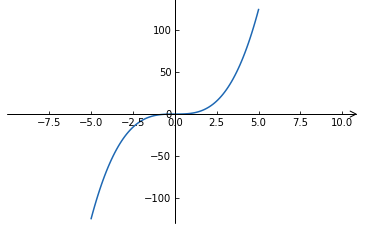
\includegraphics[scale=0.4]{odd_func.png}\\
    }
    \subfigure[偶函数]{
        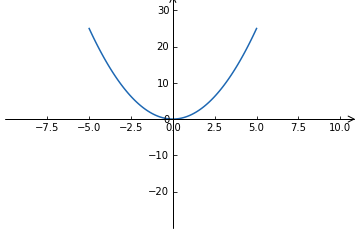
\includegraphics[scale=0.4]{even_func.png}\\
    }
\end{figure}
2.有理函数(特例$\frac{1}{x^n}$)\\
\begin{figure}[H]
    \subfigure[n为奇数]{
        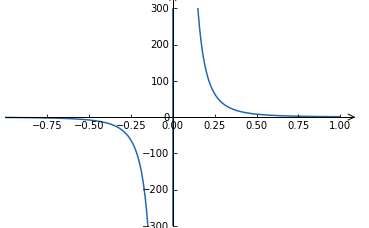
\includegraphics[scale=0.4]{odd_rati_func.png}\\
    }
    \subfigure[n为偶数]{
        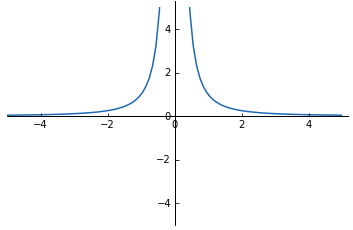
\includegraphics[scale=0.4]{even_rati_func.png}\\
    }
\end{figure}
\end{document}
